\paragraph{Sơ đồ tuần tự luồng tải lên và cập nhật ảnh đại diện}

Luồng nghiệp vụ này mô tả
quy trình người dùng
tải ảnh đại diện lên bộ lưu trữ
của Supabase và
cập nhật lại đường dẫn hình ảnh
trong hồ sơ của mình.

\subparagraph{Mô tả tổng quan}

\begin{itemize}

\item \textbf{Tải ảnh lên kho chứa:}
Người dùng chọn tải lên tệp ảnh đại diện mới hoặc URL tệp ảnh.
Giao diện tạo tên tệp ngẫu nhiên theo định danh người dùng
và gửi tệp ảnh qua cổng API đến kho lưu trữ Supabase
để lưu vào thư mục ảnh đại diện.

\item \textbf{Cập nhật thông tin tài khoản:}
Sau khi tải tệp lên kho lưu trữ Supabase thành công,
giao diện thiết lập liên kết ảnh công khai mới
và gửi yêu cầu cập nhật liên kết ảnh đại diện này qua cổng API đến CSDL thông tin cá nhân của người dùng.
\end{itemize}

\begin{figure}[H]
\centering
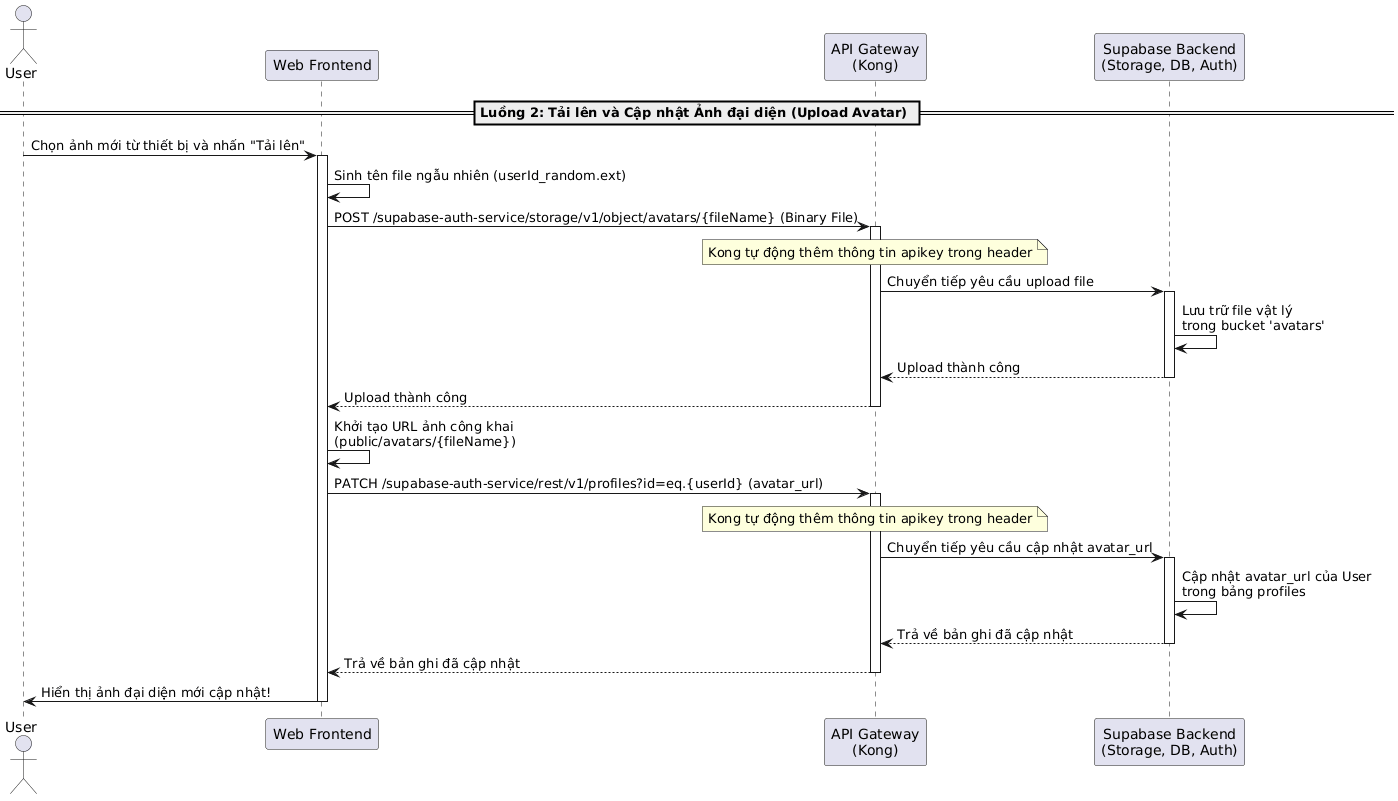
\includegraphics[width=0.95\textwidth]{contents/Sequence/UML-Sequence-UserProfileUploadAvatar.png}
\caption{Sơ đồ tuần tự luồng tải lên và cập nhật ảnh đại diện}
\end{figure}

\begin{table}[H]
\centering
\renewcommand{\arraystretch}{1.3}

\begin{tabular}{|l|l|p{5cm}|}
\hline
\textbf{Thành phần} & \textbf{Phân loại} & \textbf{Vai trò trong hệ thống} \\ \hline
User & Actor & Người dùng thực hiện chọn ảnh và lưu ảnh đại diện mới. \\ \hline
Web Frontend & Component & Giao diện web Next.js. \\ \hline
API Gateway (Kong) & Component & Cổng API chuyển tiếp các yêu cầu API. \\ \hline
Supabase Backend & Component & Dịch vụ tích hợp quản lý lưu trữ tệp tin, CSDL và xác thực. \\ \hline
\end{tabular}
\caption{Các thành phần tham gia luồng tải lên và cập nhật ảnh đại diện}
\end{table}
